\chapter{Lecture \thechapter{} of 25/03/2026}

\begin{proposition}
    
    Let $f : \Rn \to \Rb$ a function. Then 

    \begin{enumerate}
        \item[a)] $\cl{f}$ is the greatest closed function below $f$ (recall that we say $g \le f$ if $g(x) \le f(x)$ for any $x$);
        \item[b)] $\ccl{f}$ is the greatest convex closed function below $f$. 
    \end{enumerate}

\end{proposition}

\begin{proof}
    
    Let $f : \Rn \to \Rb$ closed below $f$, then $\epi{f} \seq \epi{g}$, but $\epi{\cl{f}} = \cl{\epi{f}} = $ intersection of all closed sets containing $\epi{f}$. Notice that $\epi{g}$ is closed, as $g$ is closed. Hence $\cl{\epi{f}} \seq \epi{g}$ as $\epi{g}$ is one of the closed sets containing $\epi{f}$. This shows that $\cl{f} \le g$. The same argument works for b).

\end{proof}

\section{Recession cones}

\begin{definition}[Recession direction/cone]

    Let $C$ be convex and nonempty. We say that a direction $d \in \Rn$ is a \emph{recession direction} for $C$ if $x + \alpha d \in C$ for any $x \in C$, $\alpha \ge 0$.

    We denote with $\Rc{C}$ the \emph{recession cone} of $C$ the set of all recession directions.

\end{definition}

\begin{figure}
    \centering
    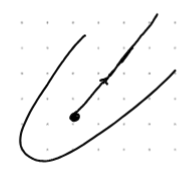
\includegraphics[width=0.7\textwidth]{img/recessionC.png}
    \caption{Example of recession cone}
\end{figure}

\begin{example}

    \begin{align}
        C &= \set{(x,y) \in \R^2 : x^2 + y^2 \le 1}. \quad \Rc{C} = \set{0}. \\
        C &= (-\infty,2]. \quad \Rc{C} = (-\infty,0].
    \end{align}
    
\end{example}

\begin{proposition}[Recession cone theorem]

    Let $C$ closed convex nonempty. Then 
d functions. This methodology is fundamental
in several convex optimization contexts, including the issue of existence of
optimal solutions, which will be discu
    \begin{enumerate}
        \item[a)] $\Rc{C}$ is closed and convex;
        \item[b)] $d \in \Rc{C} \iff$ there exists $x \in C$ such that $x + \alpha d \in C$ for all $\alpha \ge 0$.
    \end{enumerate}
    
\end{proposition}

\begin{proof}
    
    We first prove convexity. Let $d_1, d_2 \in \Rc{C}$, $\gamma_1,\gamma_2 \in [0,1]$ ssuch that $\gamma_1 + \gamma2 = 1$. Fix any $x \in C,\,\alpha \ge 0$ and consider $x + \alpha(\gamma_1 d_1 + \gamma_2 d_2) = x(\gamma_1 + \gamma_2) + \alpha(\gamma_1 d_1 + \gamma_2 d_2) = \gamma_1(x + \alpha d_1) + \gamma_2(x + \alpha d_2)$ which is a convex combination of points in $C$. For the closerness, consider $\set{d_k}_k$ a sequence in $\Rc{C}$ such that $d_k \to d \in \Rn$. Then for any $x \in C$ and for any $\alpha\ge 0$, $x + \alpha d_k \in C \to x + \alpha d$ as $k \to +\infty$. This shows that $x + \alpha d \in C$ as $C$ is closed.

    For point b), the implication ''$\implies$'' is obvious. 

    \begin{figure}[ht!]
        \centering
        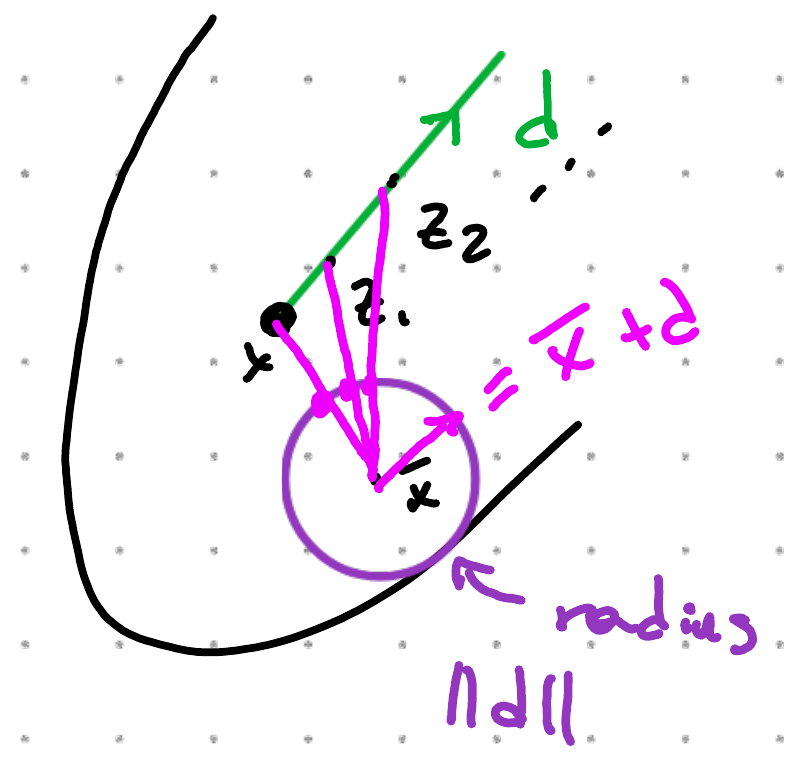
\includegraphics[width=0.5\textwidth]{img/proofRec.png}
        \caption{Visual intuition on the sequence $z_k$}
    \end{figure}

    Let $d \in \Rn$ and assume $x \in C$ such that $x + \alpha d \in C$ for any $\alpha \ge 0$. Let $\bar{x} \in C$. We have to prove $\bar{x} + \alpha d \in C$. Assume, without loss of generality, $\alpha = 1$ as we can retrive the general case with a scaling argument. Define a sequence $z_k = x + kd$, $z_k \in C$ for all $k$. If $\bar{x} = z_k$ for some $k$ then we are done. Assume then $\bar{x} \neq x_k$ and define $d_k \displaystyle\frac{z_k -\bar{x}}{\norm{z_k - \bar{x}}} \norm{d}$. Then 

    \begin{align*}
        d_k &= \frac{z_k -\bar{x} + x - x}{\norm{z_k - \bar{x}}} \norm{d} = \frac{\overbrace{z_k - x}^{= kd}}{\norm{z_k - \bar{x}}}\norm{d} + \frac{x - \bar{x}}{\norm{z_k - \bar{x}}} \\
        &= \frac{k\norm{d}}{\norm{z_k - \bar{x}}}d + frac{x - \bar{x}}{\norm{z_k - \bar{x}}}. 
    \end{align*}

    The last term goes to 0, indeed, $x - \bar{x}$ is fixed, $\norm{d}$ is fixed and $\norm{z_k} \nearrow +\infty$ as $k \nearrow +\infty$. I claim that the first term goes to $d$: in fact,

    \[ \frac{k\norm{d}}{\norm{x + kd - \bar{x}}} = \frac{k\norm{d}}{k \norm{d + (x - \bar{x})/k}} \to 1. \]

    This shows that $d_k \to d$ as $k \nearrow +\infty$. For $k$ large enough, the vector $\bar{x} + dk$ belongs to the segment connecting $\bar{x}$ to $z_k$, so, by convexity of $C$, $\bar{x} + d_k \in C$, hence $\bar{x} + d \in C$ as $C$ is closed.

\end{proof}

\begin{proposition}[Properties of the recession cone]
    
    Let $C \seq \Rn$ closed convex nonempty. Then 

    \begin{enumerate}
        \item[a)] $\Rc{C}$ contains a nonzero direction if and only if $C$ is unbounded;
        \item[b)] $\Rc{C} = \Rc{\ri{C}}$
        \item[c)] if $\set{C_i}_{i \in I}$ is a collection of closed convex sets such that $\displaystyle\bigcap_{i \in I} C_i \neq \emptyset$, then $\Rc{\bigcap_i C_i} = \bigcap_{i \in I} \Rc{C_i}$;
        \item[d)] fix $W \seq \Rn$ compact, $A \in \R^{n\times n}$ a matrix. Let $V = \set{x \in C : Ax  \in W}$. Assume $V$ nonempty. Then $\Rc{V} = \Rc{C} \cap N(A)$ where $N(A) = \set{x \in \Rn : Ax = 0}$ is the null space of the linear operator $A$.
    \end{enumerate}

\end{proposition}

\begin{proof}
    Not required.
\end{proof}

\begin{example}

    The following example shows how the closerness of $C$ can play a role in the recession cone. Consider the set 

    \[ C = \set{(x,y) \in \R^2 : 0 \le x \le 1,\, y \ge 0} \cup \set{(1,0)}. \]

    Then $\Rc{C} = \set{0}$, indeed, if we start from the point $(1,0)$, we cannot move along any direction without leaving $C$, while $\Rc{\ri{C}} = \mathrm{span}\set{(0,1)}$. 
    
\end{example}

\section{Linearity space}

We define the linearity space for a set $C$ as the set 

\[ \Lc{C} = \Rc{C} \cap (-\Rc{C}). \]

In other words, $d \in \Lc{C}$ if and only if $x + \alpha d \in C$ and $x - \alpha d$ are inside $C$ for any $\alpha \ge 0$.

\begin{proposition}[Properties of $\Lc{C}$]
    
    Let $C \seq \Rn$ convex closed nonempty, then 

    \begin{enumerate}
        \item $\Lc{C}$ is a subspace;
        \item $\Lc{C} = \Lc{\ri{C}}$;
        \item same as above.
    \end{enumerate}

\end{proposition}

\begin{proof}
    Not required.
\end{proof}

\begin{example}[Important!]
    
    Consider the set 

    \[ C = \set{x \in \Rn : x^\top Q x + c^\top x + b \le 0} \]

    where $Q \in \R^{n \times n}$ is SPD, $c \in \Rn$, $b \in \R$. We want to compute $\Rc{C}$.

    Let $x \in C$, $d \in \Rn$. Then $x + \alpha d \in C$ for any $\alpha \ge 0$ if and only if 

    \begin{align*}
        &(x + \alpha d)^\top Q (x + \alpha d) + c^\top (x + \alpha d) + b \le 0 \\
        &\iff \underbrace{x^\top Q x + c^\top x + b}_{\le 0} + \alpha(c^\top d + 2x^\top Q)d + \alpha^2 d^\top Q d \le 0  
    \end{align*}

    for any $\alpha \ge 0$ and for any $x \in C$.

    The quantity $\alpha^2 d^\top Q d \ge 0$ since $Q$ is SPD, hence we need $d^\top Q d = 0$. Since $Q$ is SPD, we can compute its Cholesky factorization, hence $Q = M^\top M \implies d^\top M^\top M d = 0$, so $Md = 0$. 

    Furthermore, we need also $\alpha c^\top d \le 0$. Finally, the recession cone turns out to be 

    \[ \Rc{C} = \set{d \in \Rn : Qd = 0,\, c^\top d \le 0}. \]

    Moreover, 

    \[ \Lc{C} = \set{d \in \Rn : Qd = 0,\, c^\top d = 0}. \]

\end{example}